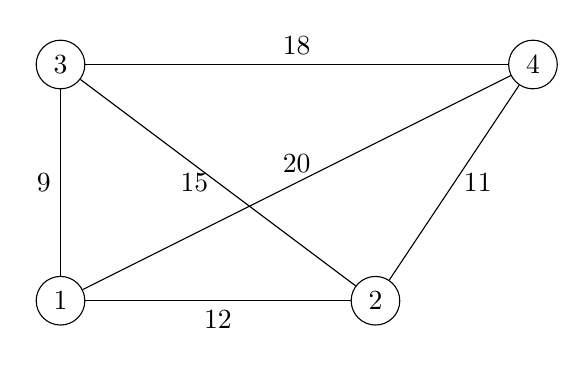
\begin{tikzpicture}
 \node[circle,draw] (A) at (0,0) {1};
 \node[circle,draw] (B) at (4,0) {2};
 \node[circle,draw] (C) at (0,3) {3};
 \node[circle,draw] (D) at (6,3) {4};

 \draw (A) -- node[midway, below] {12} (B); 
 \draw (A) -- node[midway, left] {9} (C);
 \draw (A) -- node[midway, above] {20} (D);
 \draw (B) -- node[midway, left] {15} (C);
 \draw (B) -- node[midway, right] {11} (D);
 \draw (C) -- node[midway, above] {18} (D); 
\end{tikzpicture}
